\documentclass[12pt]{article}
%\usepackage{times}
\usepackage{cite}
\usepackage{indentfirst}
\usepackage{graphicx}
\usepackage{subcaption}
%this is a comment
\title{Project Proposal: Volunteer Connector}
\author{Daniel Domme (onid: dommed) \\and Charles Koll (onid: kollch)}
\date{13 February 2018}




\begin{document}
\maketitle
\tableofcontents



\section{Volunteer Connector}
\subsection{Introduction and Need}
 In the United States of America, there are many charitable organizations or causes that need the help of volunteer citizens to make a better world a reality.  At the same time, there are many people who would like to help out, but they are not sure where to help or how.  According to the Bureau of Labor Statistics, volunteering went gone down by .4 percent to to 24.9 percent in 2015.\cite{bls}  There needs to be a change that increases the visibility of volunteer positions.  Our team, Volunteer Benevolence, has come up with the idea of a new website called Volunteer Connector to help increase awareness.  The website would solve the problem of a lack of connection and communication/advertisement between volunteer organizations and potential volunteers.  Right now, there is a lack of free central site for charitable organizations to post a need for volunteers and for volunteers to search for positions at charitable organizations, and our website idea could solve it.\\

\subsection{Evidence}
Experience by group member, Daniel Domme, has shown that it is hard to find what opportunities are available in the local community to volunteer for that match personal needs. In an article on the website WiredImpact.com says, ``Since there are tons of nonprofits finding a volunteer opportunity is pretty easy to do.  The issue is finding an opportunity that fits your needs and interests.'' \cite{volwebsite} A quick search for ``recruit volunteers'' lists literature on strategies to gain volunteers for your organization, but it does not provide any good resources for advertising for free to get volunteers or charitable giving.  A second search for ``volunteer'' results in poor listing sites that are hard to navigate and do not allow users to find exactly what they are looking for.  \\

\subsection{Brief Story}
Say you’re looking to volunteer, but you don’t know what you’re looking for. You go to Google to find something, but there isn’t a site that has various opportunities, so you end up not doing anything. Now say you’re an organization that needs volunteers. You’ll need to advertise for it, which costs money, which you clearly don’t have since otherwise you’d just hire people. Since your advertising isn’t as strong as you’d like, you don’t get as many volunteers as you need.  There is clearly a disconnect between the two parties who are trying to find each other.  A simple website that is easy to use could be used to bridge the gap and improve the communities and lives of people around the country.\\

\subsection{Solution Details}
Our approach to solve the problem of lack of a central website to connect volunteers and charitable organizations is a website with a searchable database that allows volunteers to find volunteer positions with charitable events and organizations.  Volunteer organizations can post advertisements for events and positions that need to be filled and link back to their website for more information.  There will be two different account types: volunteers and organizations.  Organizations get verified outside of the site to ensure that they are legitimate causes.  This ensures the safety of the volunteer users.\\

\subsection{Uniqueness}
The main difference between our application and other approaches is that ours is free. Many others charge charitable organizations to advertise their events.  The postings will also be highly searchable to enable the matching of needs for volunteers.

\subsection{Possible Limitations}
Some limitations do exist with the chosen approach.  One such limitation is the lack of revenue to fund server costs, wages, licenses, advertising, and web traffic.  This can possibly be overcome by asking for donations and becoming a nonprofit charitable organization.  Another limitation would be the lack of ability to verify volunteer identities.  It should not be too large of a problem as the site is mainly a place to post volunteer opportunities.  The final limitation is the amount of time to complete and implement features on the website.  The short amount of time given to complete this project might inhibit the functionality and finish of the service provide by the website.
Resources that are needed for this project include a database, server space, development software, development computers, and github.  A linux environment will also be preferred to develop the website.  Team planning and design will need to be completed prior to the start of implementing ideas.\\

\subsection{Needed Resources}
Many challenges may be faced during the development of this website.  A major one is implementing the two different account types:  volunteer and charitable organization.  Charitable organizations will need to be verified for correct identity before they can make new posts for opportunities.  Volunteers will only need to register and browse opportunities.  They possibly will need a place to save opportunities.  Another challenge will be making volunteer opportunity postings searchable.  This will require a well thought out design and will require time to implement.  Risks will be mitigated by splitting up parts of the project to different team members to be able to implement all feature on time.  Delegating among team members will also allow for features to be developed concurrently, which means that any problems between features will be identified as soon as they are developed.  The use of content tags that will be searchable in the database will also be required by the job poster in order to allow for volunteers to find what they are looking for.  Finally, verifying charitable organizations will help to protect volunteer safety.\\

\subsection{Conclusion}
The website that our group is proposing is intended to provide a central website for volunteers to find opportunities and charities to advertise those opportunities.  It will be free for all involved and will be easy to use.  This will hopefully improve the world around us by getting more people involved with their communities. It is this group’s hope that this will increase everyone’s stake in the health and happiness of the world.  

%\subsection{Bold Text}
%{\bf Hello, world!}
%\subsubsection{Bold and Large Text}
%{\Large \bf Hello, world!!!}

\section{Presentation Slides}
What follows are our group's presentation slides.
\begin{figure}
  \centering
  \begin{subfigure}[b]{0.7\linewidth}
    
\includegraphics[width=\linewidth]{slide1}
  \end{subfigure}
  \begin{subfigure}[b]{0.7\linewidth}
    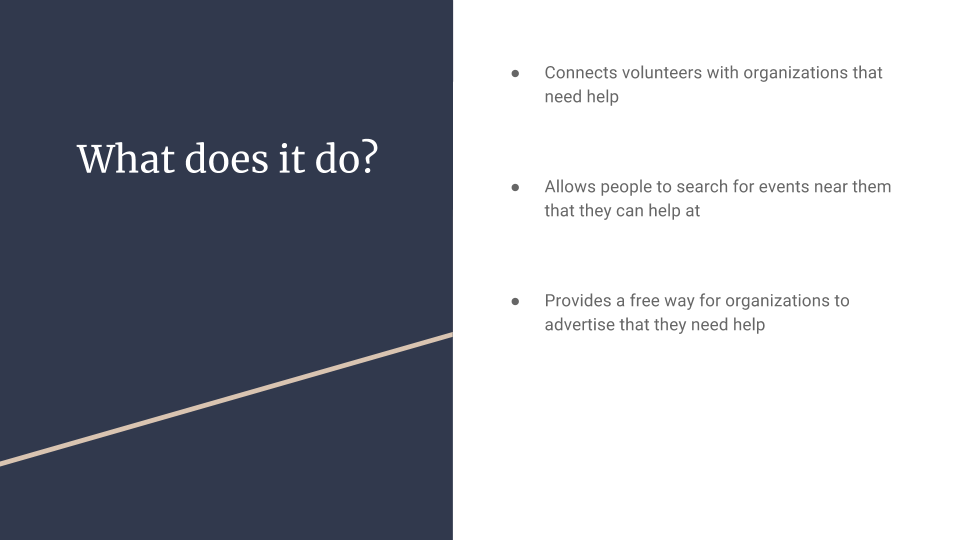
\includegraphics[width=\linewidth]{slide2}
  \end{subfigure}
  \begin{subfigure}[b]{0.7\linewidth}
    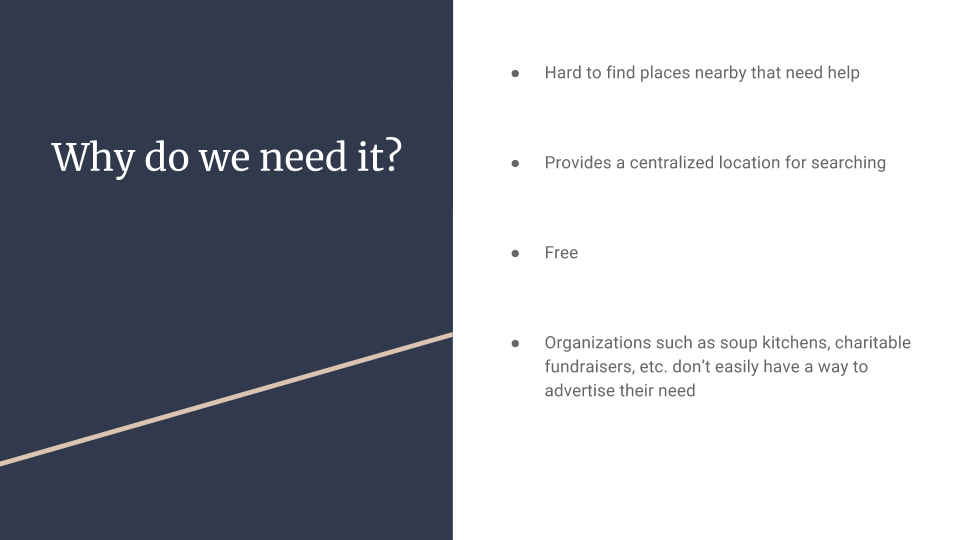
\includegraphics[width=\linewidth]{slide3}
  \end{subfigure}
\end{figure}
\clearpage
%Software Engineering: Theory and Practice~\cite{pfleeger2010software}

%Software Engineering~\cite{sommerville2011software}


\bibliography{myref}
\bibliographystyle{unsrt}

\end{document}
